\documentclass[border=6mm]{standalone}
\usepackage[T1]{fontenc}
\usepackage[default,semibold]{sourcesanspro}
\usepackage{xcolor}
\usepackage{tikz}
\usetikzlibrary{positioning,shapes.geometric,shapes.symbols,arrows.meta,calc,fit,backgrounds}

\definecolor{navy}{HTML}{1C3A5E}
\definecolor{pblue}{HTML}{3B78B5}
\definecolor{amber}{HTML}{F2B33D}
\definecolor{deepamber}{HTML}{D9902A}
\definecolor{pale}{HTML}{EEF3F9}
\definecolor{ink}{HTML}{2A2F36}
\definecolor{soft}{HTML}{5E6773}

\tikzset{
	every node/.style={font=\small, text=ink},
	step/.style={draw=navy, line width=0.8pt, rounded corners=3pt, fill=white, align=center, text width=#1, inner sep=6pt, minimum height=11mm},
	step/.default=44mm,
	optstep/.style={step=#1, dashed},
	optstep/.default=44mm,
	input/.style={draw=deepamber, line width=0.8pt, rounded corners=3pt, fill=amber!18, align=left, text width=48mm, inner sep=6pt},
	decision/.style={diamond, aspect=1.9, draw=navy, line width=0.8pt, fill=pale, align=center, text width=34mm, inner sep=1pt},
	store/.style={cylinder, shape border rotate=90, aspect=0.18, draw=navy, line width=0.8pt, fill=navy, text=white, align=center, text width=40mm, minimum height=19mm, inner sep=4pt},
	flow/.style={-{Stealth[length=2.6mm]}, line width=0.8pt, draw=navy},
	optflow/.style={flow, dashed},
	label/.style={font=\footnotesize\itshape, text=soft},
	stage/.style={draw=none, fill=pale, rounded corners=6pt, inner sep=5mm},
	stagetitle/.style={font=\bfseries\large, text=navy, anchor=north west},
}

\begin{document}
\frenchspacing
\hyphenpenalty=10000
\exhyphenpenalty=10000
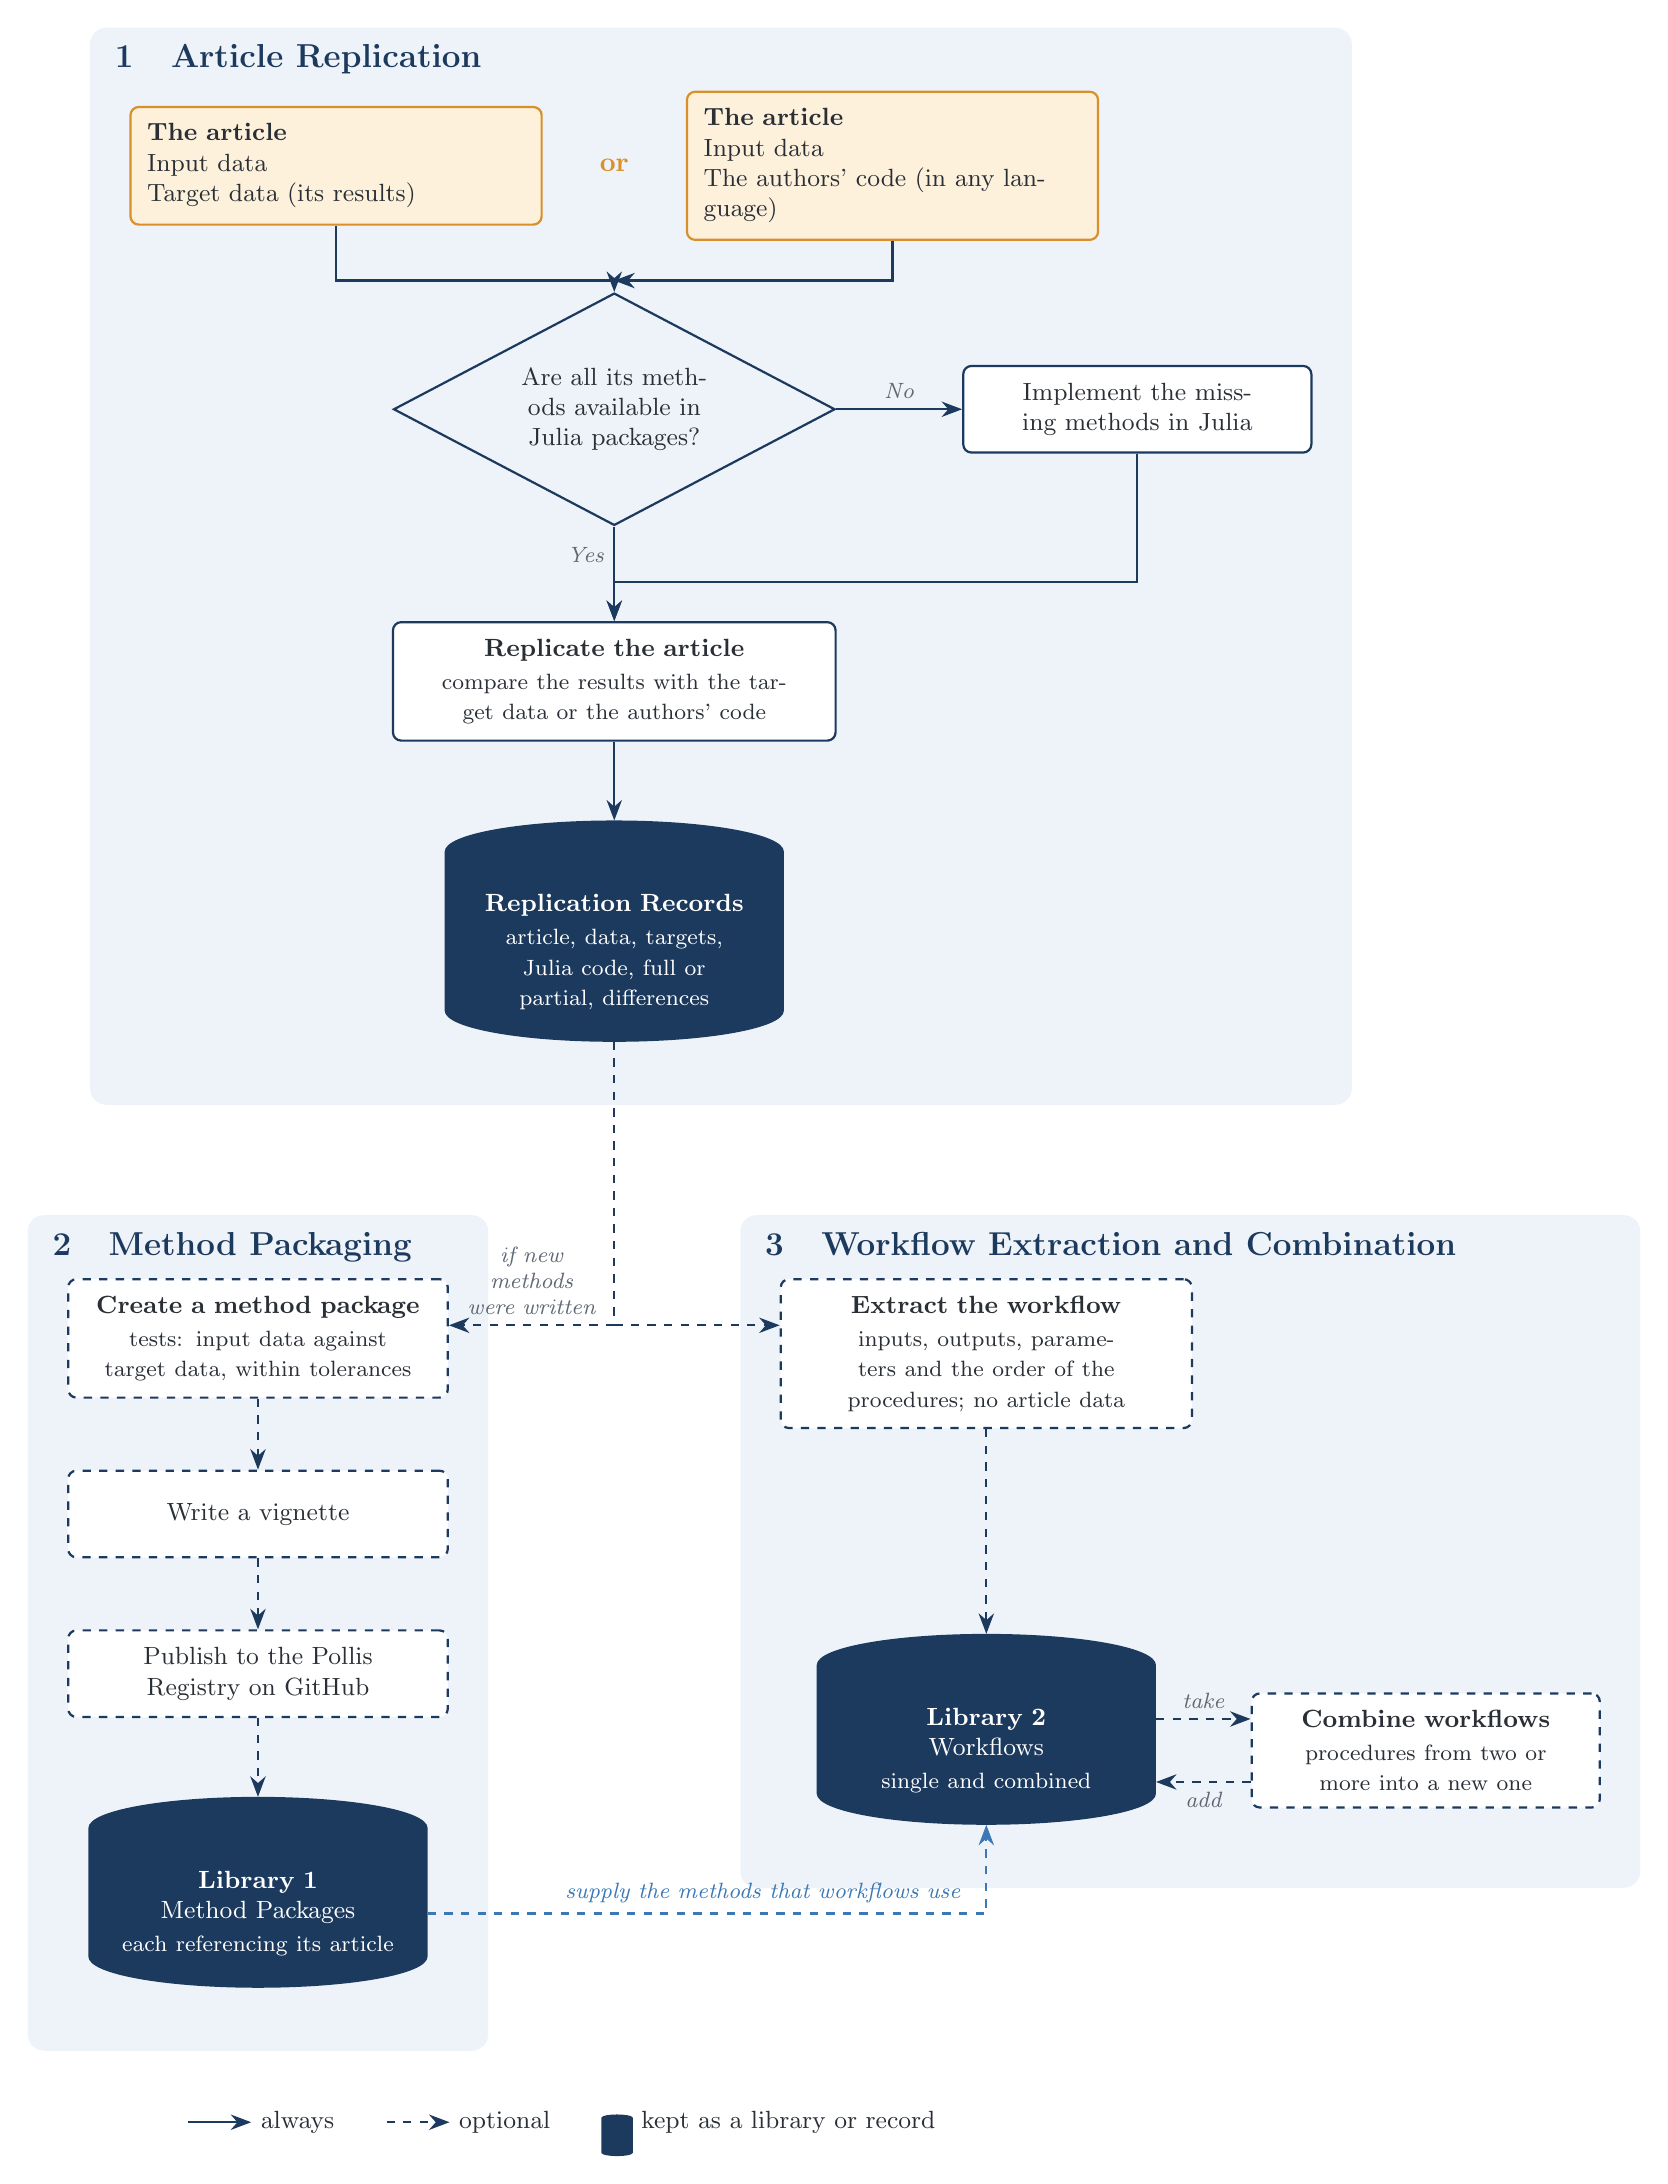
\begin{tikzpicture}[node distance=9mm and 10mm]

% ---------- 1. Article Replication ----------
\node[input] (in1) {\textbf{The article}\\Input data\\Target data (its results)};
\node[font=\bfseries, text=deepamber, right=6mm of in1] (or) {or};
\node[input, right=6mm of or] (in2) {\textbf{The article}\\Input data\\The authors' code (in any language)};

\coordinate (merge) at ($(in1.south)!0.5!(in2.south) + (0,-6mm)$);
\node[decision, below=14mm of or] (avail) {Are all its methods available in Julia packages?};
\node[step=40mm, right=16mm of avail] (implement) {Implement the missing methods in Julia};
\node[step=52mm, below=12mm of avail] (replicate) {\textbf{Replicate the article}\\[1pt]\footnotesize compare the results with the target data or the authors' code};
\node[store, below=10mm of replicate] (records) {\textbf{Replication Records}\\[1pt]\footnotesize article, data, targets, Julia code, full or partial, differences};

\draw[flow] (in1.south) |- (merge) -- (avail.north);
\draw[flow] (in2.south) |- (merge);
\draw[flow] (avail.east) -- node[label, above] {No} (implement.west);
\draw[flow] (avail.south) -- node[label, left, pos=0.3] {Yes} (replicate.north);
\draw[flow] (implement.south) |- ($(replicate.north)+(0,5mm)$) -- (replicate.north);
\draw[flow] (replicate) -- (records);

% ---------- 2. Method Packaging ----------
\node[optstep, anchor=north east] (package) at ($(records.south)+(-21mm,-30mm)$) {\textbf{Create a method package}\\[1pt]\footnotesize tests: input data against target data, within tolerances};
\node[optstep, below=of package] (vignette) {Write a vignette};
\node[optstep, below=of vignette] (publish) {Publish to the Pollis Registry on GitHub};
\node[store, below=10mm of publish] (packages) {\textbf{Library 1}\\Method Packages\\[1pt]\footnotesize each referencing its article};

% After a replication, both next steps are optional and independent
\coordinate (split) at ($(records.south)+(0,-36mm)$);
\draw[optflow, -] (records.south) -- (split);
\draw[optflow] (split) -- node[label, above, text width=17mm, align=center] {if new methods were written} (split -| package.east);
\draw[optflow] (package) -- (vignette);
\draw[optflow] (vignette) -- (publish);
\draw[optflow] (publish) -- (packages);

% ---------- 3. Workflow Extraction and Combination ----------
\node[optstep=48mm, anchor=north west] (extract) at ($(records.south)+(21mm,-30mm)$) {\textbf{Extract the workflow}\\[1pt]\footnotesize inputs, outputs, parameters and the order of the procedures; no article data};
\node[store, below=26mm of extract] (workflows) {\textbf{Library 2}\\Workflows\\[1pt]\footnotesize single and combined};
\node[optstep=40mm, right=12mm of workflows] (combine) {\textbf{Combine workflows}\\[1pt]\footnotesize procedures from two or more into a new one};

\draw[optflow] (split) -- (split -| extract.west);
\draw[optflow] (extract) -- (workflows);
\draw[optflow] ($(workflows.east)+(0,4mm)$) -- node[label, above] {take} ($(combine.west)+(0,4mm)$);
\draw[optflow] ($(combine.west)+(0,-4mm)$) -- node[label, below] {add} ($(workflows.east)+(0,-4mm)$);

% Libraries are connected: packages supply the methods that workflows use
\draw[optflow, draw=pblue] (packages.east) -| node[label, above, pos=0.3, text=pblue] {supply the methods that workflows use} (workflows.south);

% ---------- Stage backgrounds ----------
\begin{scope}[on background layer]
	\node[stage, fit=(in1)(in2)(implement)(records), inner ysep=8mm] (s1) {};
	\node[stage, fit=(package)(packages), inner ysep=8mm] (s2) {};
	\node[stage, fit=(extract)(workflows)(combine), inner ysep=8mm] (s3) {};
\end{scope}
\node[stagetitle] at ($(s1.north west)+(2mm,-1mm)$) {1\quad Article Replication};
\node[stagetitle] at ($(s2.north west)+(2mm,-1mm)$) {2\quad Method Packaging};
\node[stagetitle] at ($(s3.north west)+(2mm,-1mm)$) {3\quad Workflow Extraction and Combination};

% ---------- Legend ----------
\node[below=16mm of packages.south west, anchor=north west, inner sep=0] (legend) {%
	\tikz[baseline=-0.6ex]\draw[flow] (0,0) -- (8mm,0); always\qquad
	\tikz[baseline=-0.6ex]\draw[optflow] (0,0) -- (8mm,0); optional\qquad
	\tikz[baseline=-0.6ex]\node[store, text width=3mm, minimum height=5mm, inner sep=1pt] {}; kept as a library or record};

\end{tikzpicture}
\end{document}
